\newpage
\section{Exemples de tableau et figure}



% Comment incorporer une image au texte
\begin{figure}[H]
    \centering
    \caption{Exemple d'image provenant du dossier "images"}
    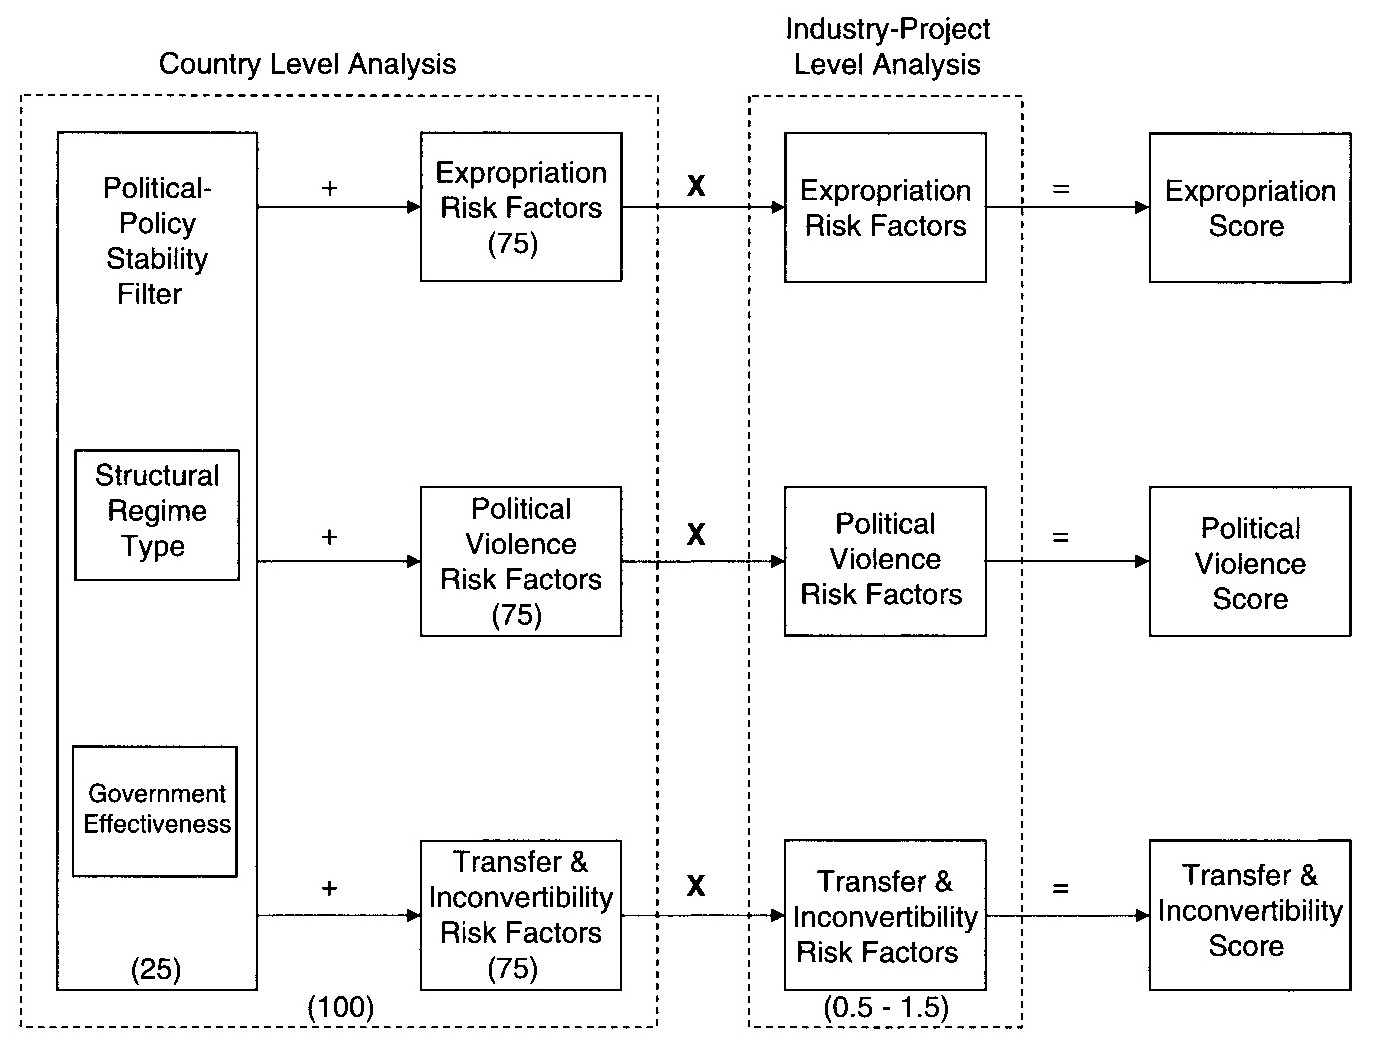
\includegraphics[keepaspectratio, width = 0.75\textwidth]{images/Schema-General.jpg}
    \source{Écrire le nom de la source en texte} % Affiche la note de référence
    \label{figure1} % Une étiquette qui permettra de référer au tableau avec un lien
\end{figure}




% Exemple de tableau
\begin{table}[ht]
    \centering % Centre le tableau dans la page
    \caption{Nonlinear Model Results}\label{tableau1} % Titre et label
    \begin{tabular}{c c c c} % Permet de créer 4 colonnes centrées
        \hline\hline \\ [-6.5ex] % Insère une ligne horizontale double
        Case & Method-1 & Method-2 & Method-3 \\ [0.5ex] % Titres des colonnes
        \hline \\ [-4.5ex] % Insère une ligne horizontale simple
        1 & 50 & 837 & 970 \\ % Insère le corps du tableau
        2 & 47 & 877 & 230 \\ % chaque colonne est séparée par un &
        3 & 31 & 25 & 415 \\
        4 & 35 & 144 & 2356 \\
        5 & 45 & 300 & 556 \\ [1ex] % Ajoute un espace vertical de "1ex" avant la ligne du bas
        \hline % Insère une ligne horizontale simple
    \end{tabular}
    
    \source{Insérer la source des données ici} % Affiche la note de référence
\end{table}